\section{Matching}%
\label{sub:alternative_matching_method}

Control group design:
\begin{itemize}

    \item We only have data for a self-selected group of people who choose to
        use the app. This has a couple consequences:

    \item By virtue of signing up to an app that helps them manage
        their money, these users are different from those who don't
        sign up. As a result, we are unable to answer the question of
        whether app use helps the average person in the
        population as a whole save more.\footnote{One way to get closer
            to that answer is to re-weight our sample on observable
            demographic variables so as to match the UK population as a
            whole. But our sample differs from the population as a
            whole both is ways that are observable (demographic
            variables) and unobservable (self-awareness that they need
            help managing their money, cognitive resources to engage
            with the app, motivation to do so). Re-weighting would only
            help us deal with the first of these.}

    \item Even among people who do eventually sign up to the app,
        hte decision when to do so is unlikely to be random --
        \textit{something} makes them sign up at the particular
        point in time they do and not before or after. If we think
        of this factor as ``motivation to save more'', then said
        motivation is inextricably linked with the decision to sign
        up so that we cannot differentiate between the two.

    \item Hence: due to the first point above, we cannot estimate
        an ATE (effect of app use on the average citizen), and due
        to the second point we also cannot estimate a pure ATT
        (effect of app use on users). Instead, our estimated effect
        of app use captures the effect of being motivated to save
        more and using the app to do so.\footnote{One way to get a
            step closer to ATT would be to find a variable that
        correlates with ``motivation to save'' and control for it /
    match on it.}

    \item This is true for both our matched DiD and our TWFE
        design. While these two approaches use a different
        counterfactual to estimate the effect of app use
        (behaviour of a matched control in the case of DiD and
        extrapolating within-user pre-signup behaviour in the case
        of TWFE), neither can help us with the fact that the
        decision to sign up is likely correlated with the
        time-varying unobserved effect ``motivation to save more''.

\end{itemize}

DiD:
\begin{itemize}

    \item We use a difference-in-differences design to estimate the effect of
        app use. Because we do not have a separate control group, we use the
        per-signup data of Money Dashboard users as control periods and use
        matching to find comparable control user for each tretment user.

    \item To do this, we use the matching estimator for panel data proposed by
        \citet{imai2021matching}. Following paper, we conduct the following
        steps:

    \item For each treated observation, we find a set of control observations
        with that share the same treatment history for a period of $L$ periods
        before the treatment and $F$ periods after the treatment. In our
        baseline specification, we rely on a year's worth of data around the
        treatment period and set $L=6$ and $F = 0, 1, 2, 3, 4, 5$.

    \item Identification assumption is that potential outcomes only depend on
        treatment status of the past L periods. In general, this means that if
        treatment has a cumulative effect over time, the full effect is reached
        after L periods. In our context, this means that any effect on savings
        behaviour from usign the app is fully realised after L periods. (I
        think this means that if we look at the treatment effect for F periods
        forward, the effect should not become stronger after F = L).

\end{itemize}

DiD identification assumptions:
\begin{itemize}
    \item No spillover effects: the potential outcome of unit $i$ at time $t$
        is independent of the treatment status of other units. This is violated
        if a user's partner or friends also use the app and, through sharing
        their experiences or motivations, influence the user's savings
        behaviour.

    \item Carryover effects no longer than $L$ periods: a user's potential
        outcome in period $t$ is independent of treatment status in periods
        more than $L$ periods ago. Given that we are dealing with an absorbing
        treatment, this is not a very strong assumption in our context, and we
        choose $L$ based on what we think is an informative number of periods
        to observe pre-app use behaviour.\footnote{An absorbing treatment is
            one that cannot be reversed, and hence we only change from
            untreated to treated once.}.

    \item Parallel trends: the spending trajectory between treated and control
        units would have continued to be parallel if the treated unit hadn't
        started using the app. This is violated whenever an intended change in
        savings behaviour also provided the impetus for the user to start using
        the app, which is likely to occurr frequently. To the extent this is
        the case, we have an ommitted variable ``motivation to save more'',
        which both changes the user's savings behaviour and their treatment
        status. Because of this, what we are measuring is not a pure ATT of app
        use -- the effect of app use on savings over and above the change
        precipitated by a change motivation -- but the effect of app use for
        users motivated to save more.

\end{itemize}


\begin{figure}[H]
    \centering
    \caption{Match set examples}%
    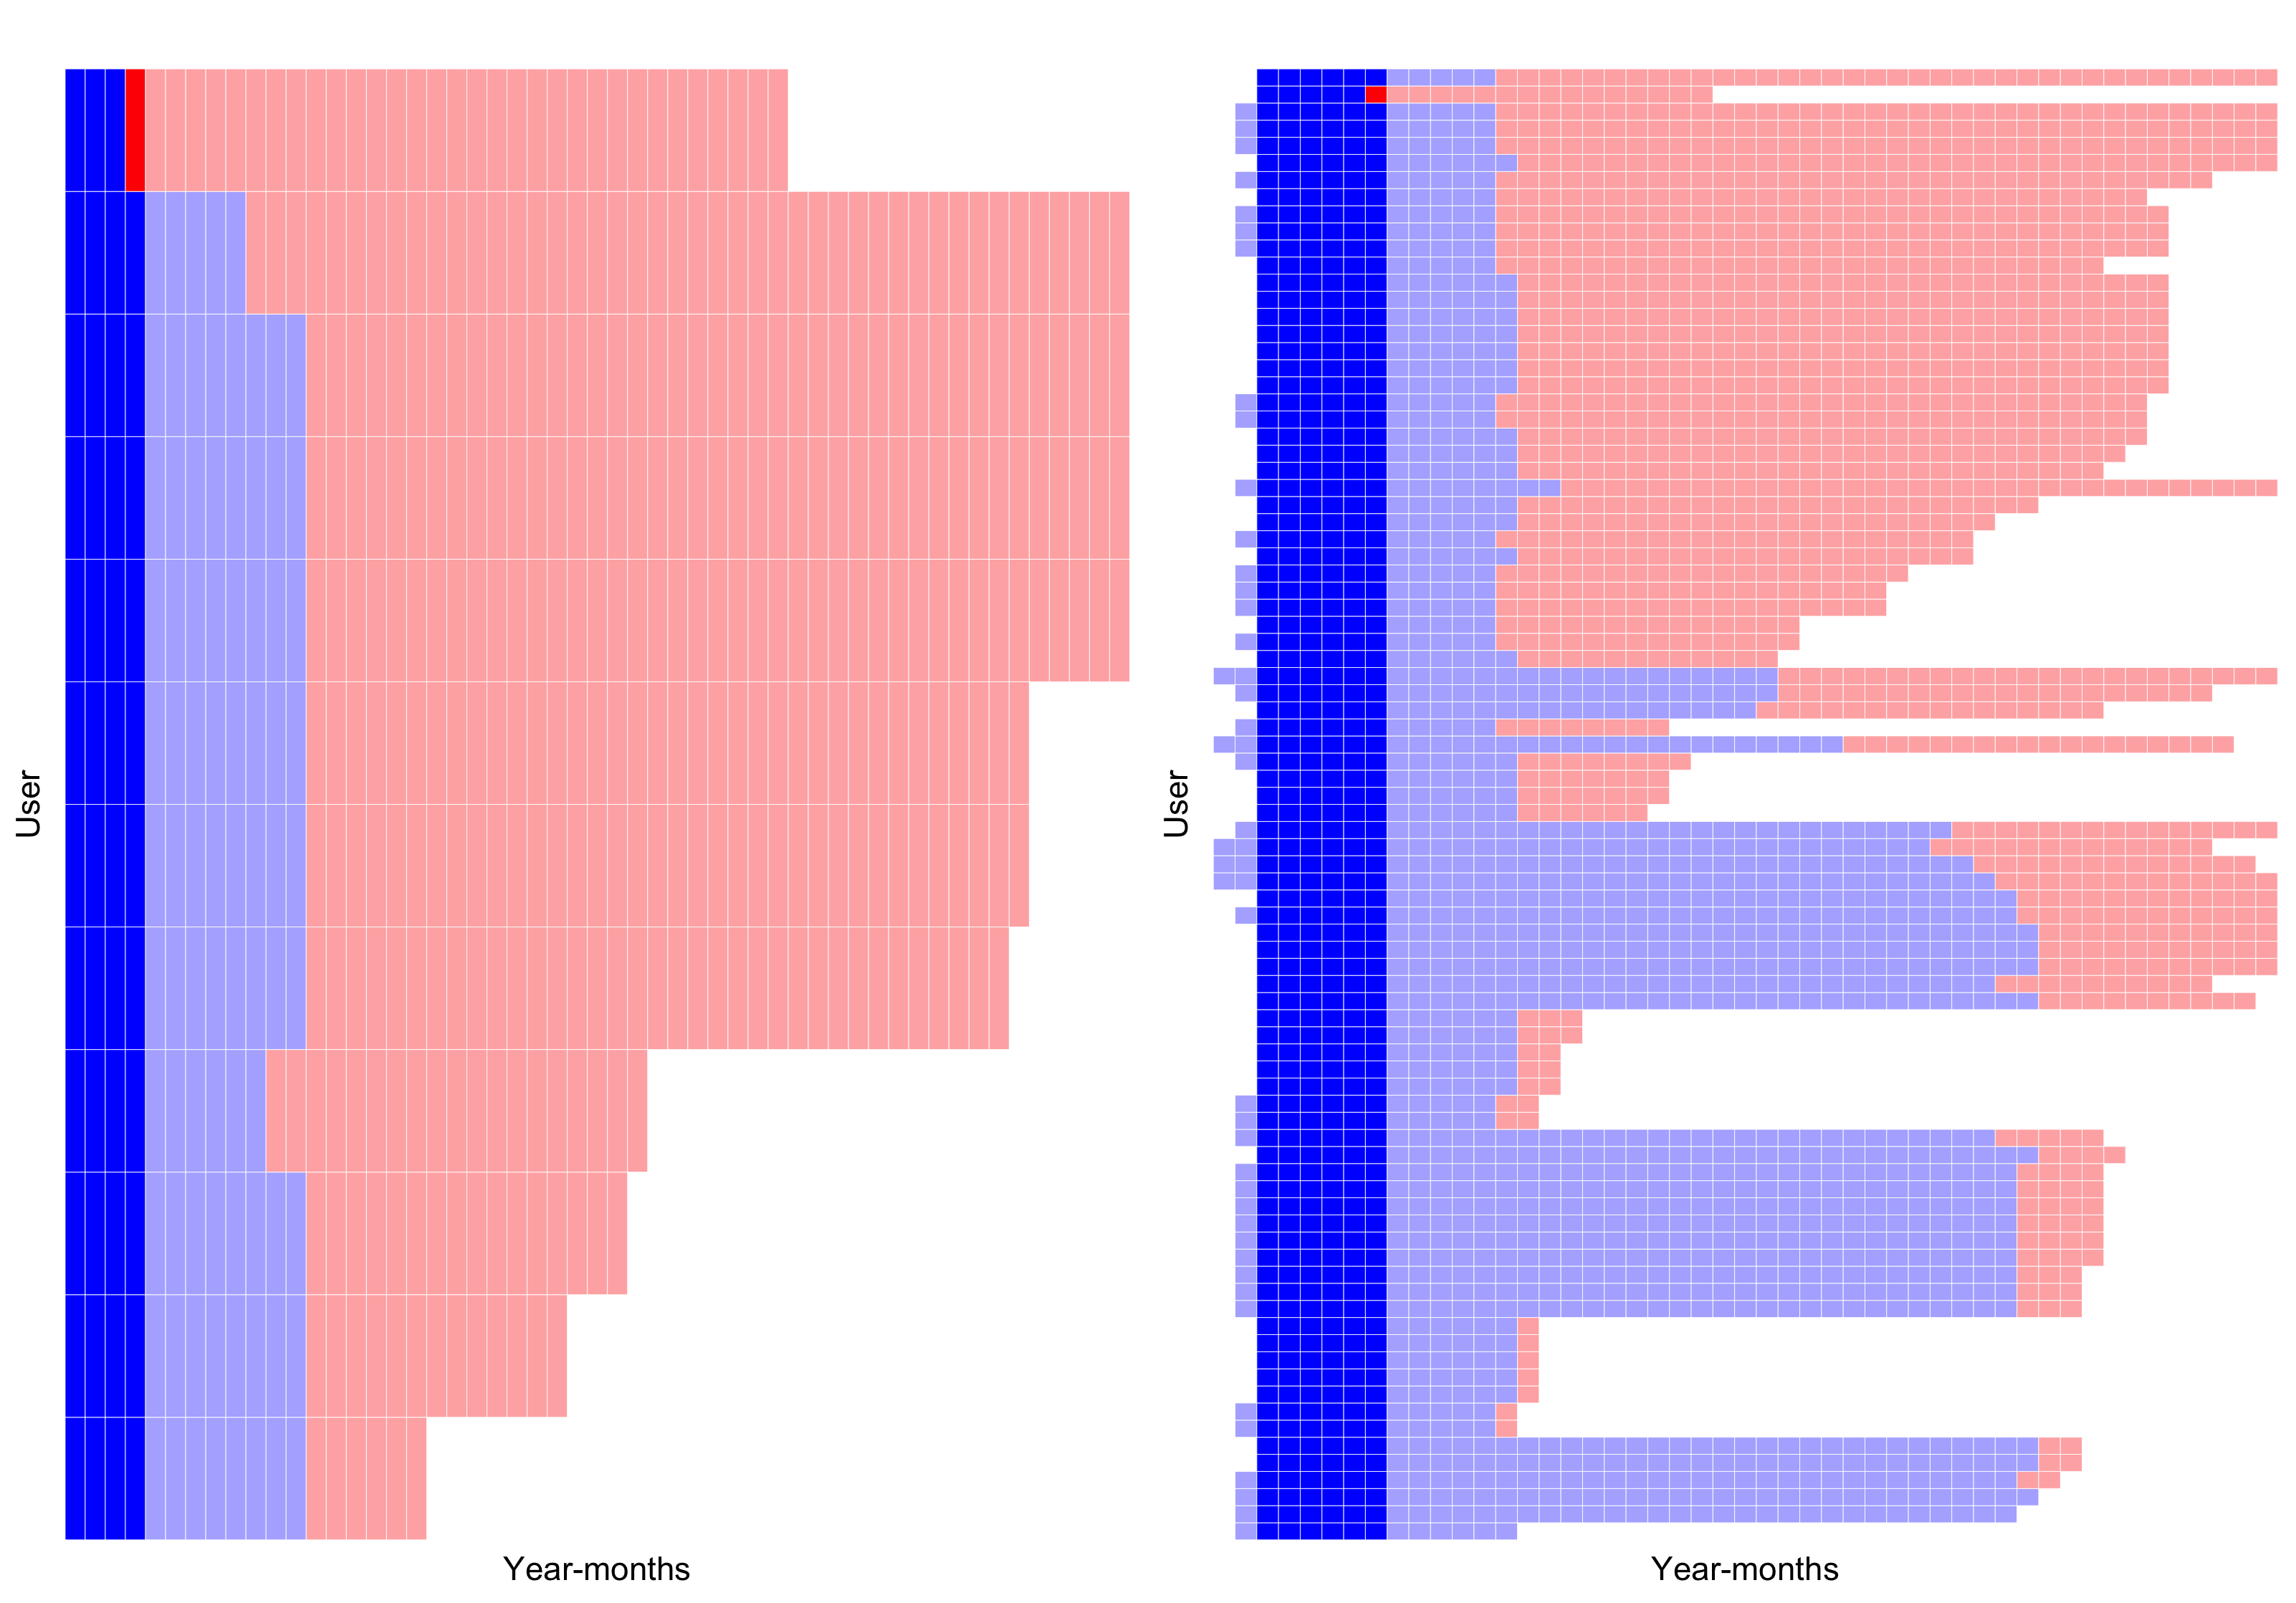
\includegraphics[width=\linewidth]{\figdir/matchset_examples.png}
    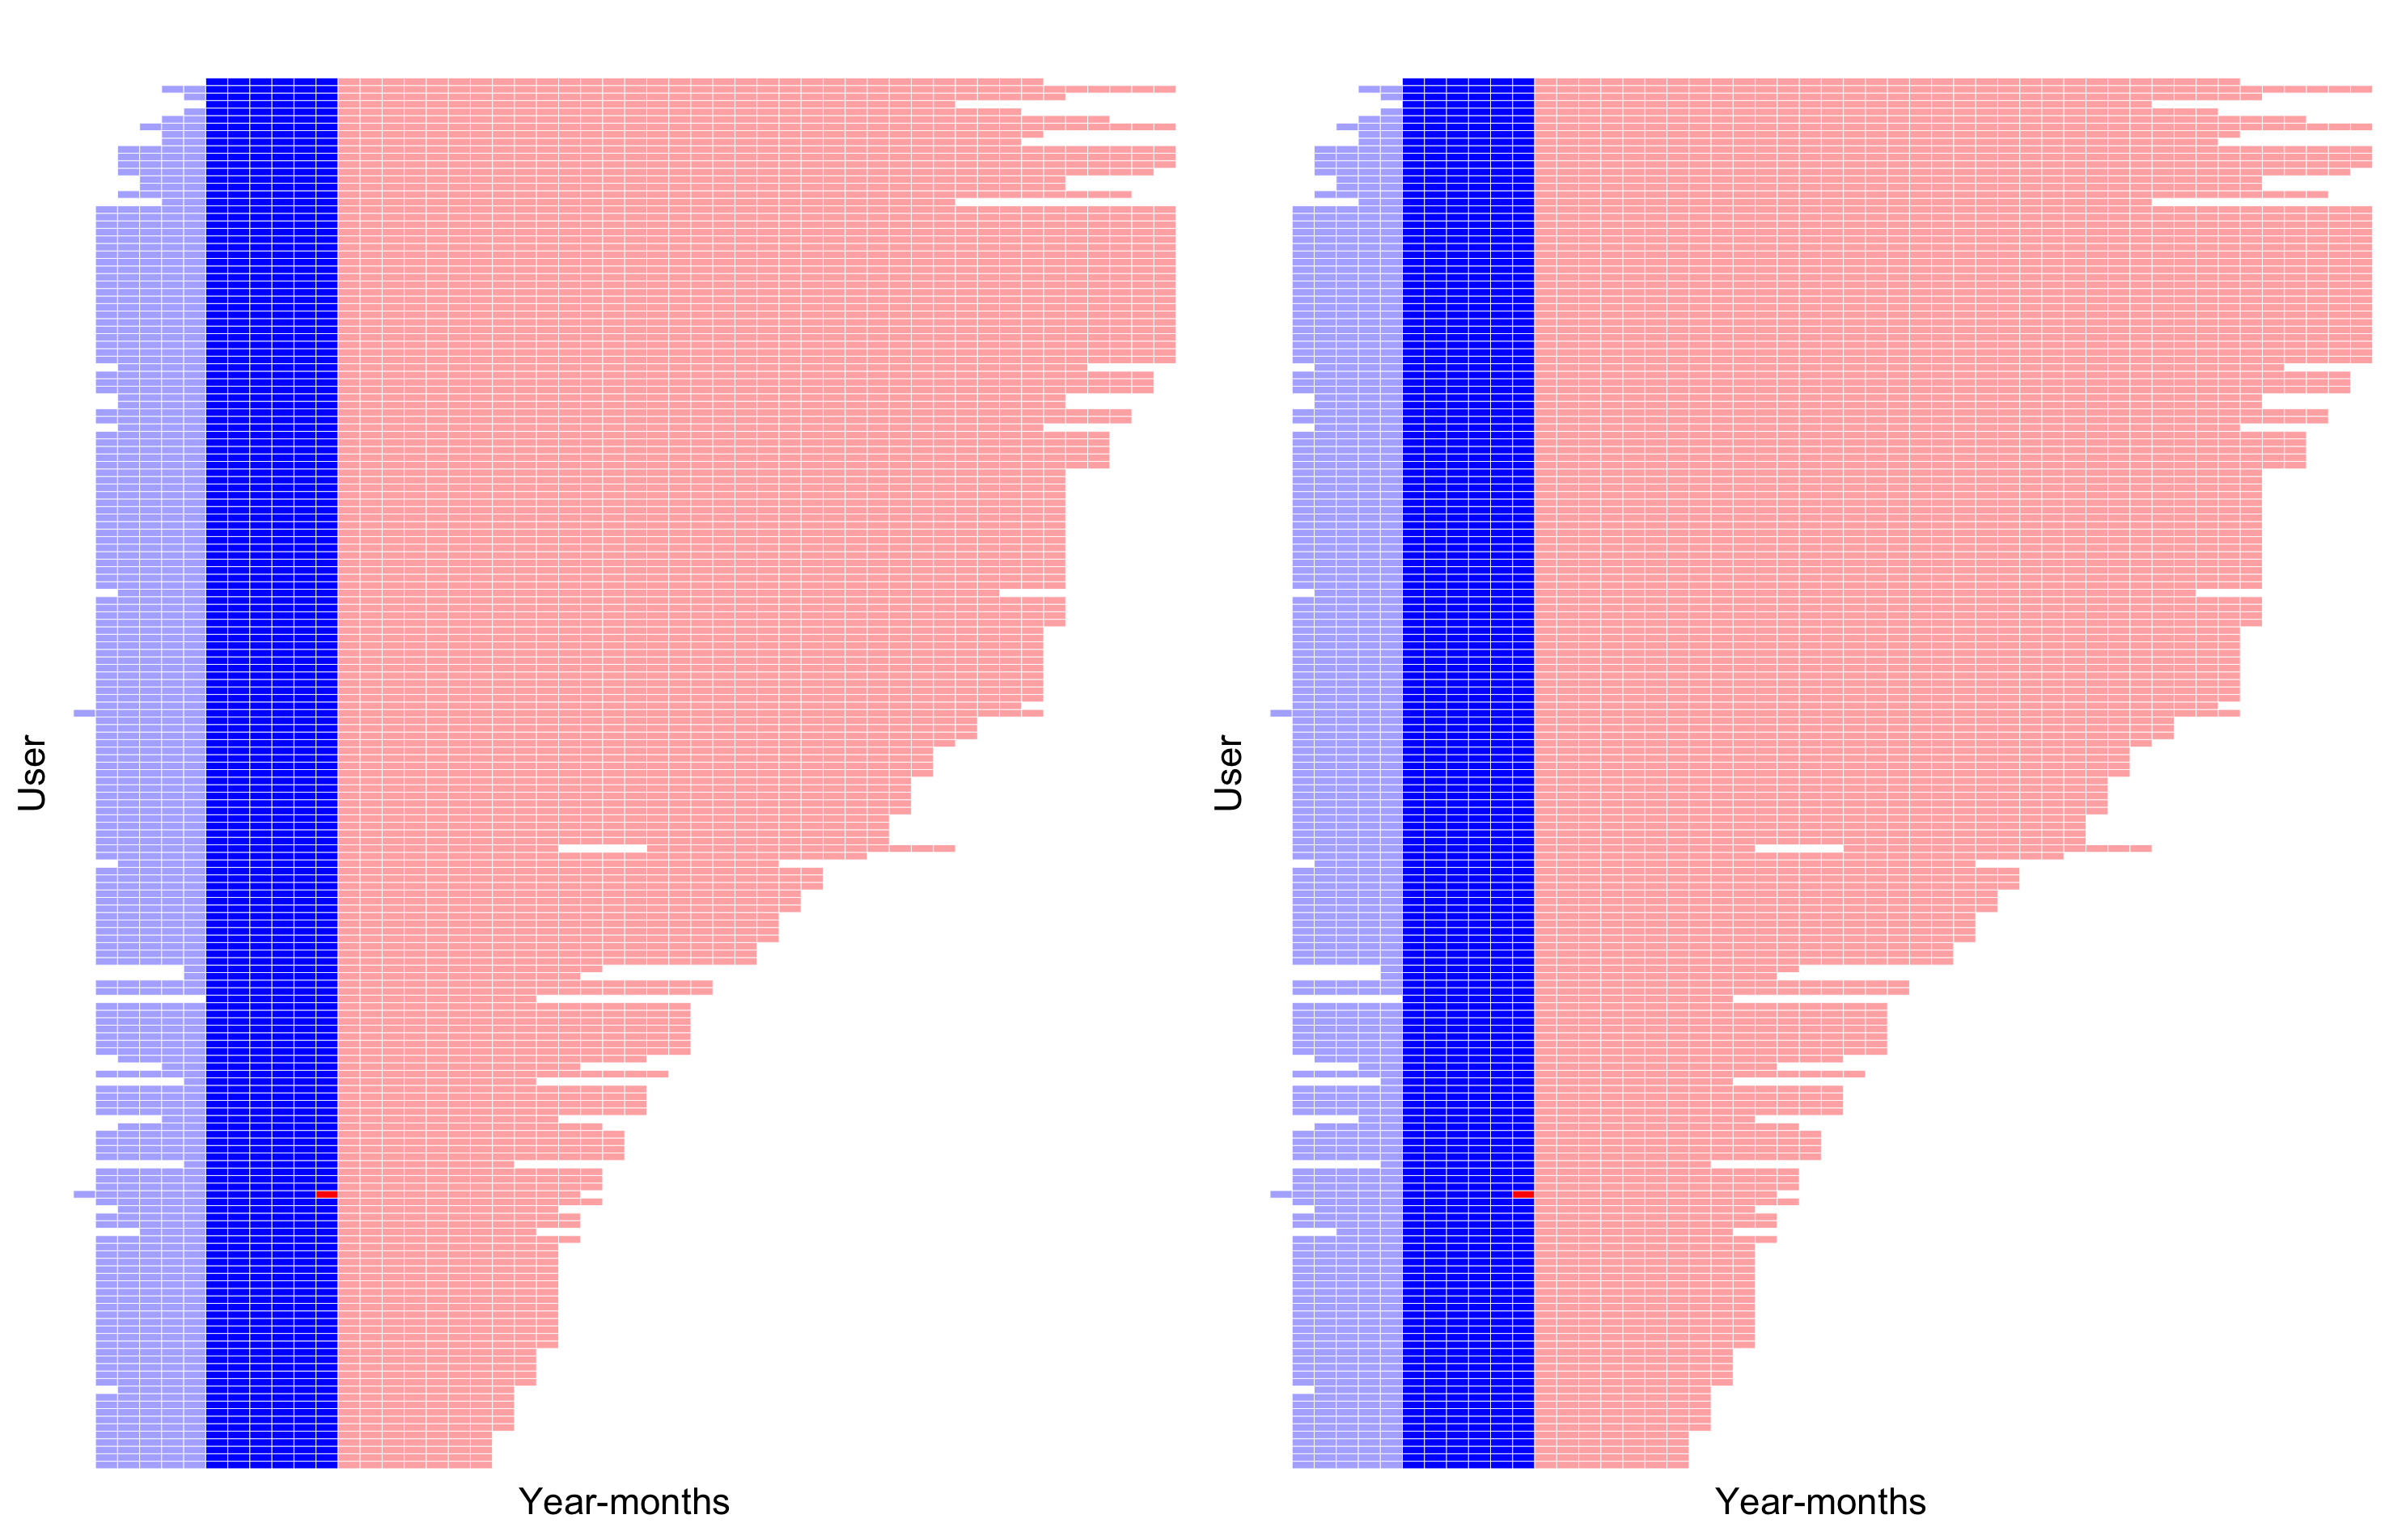
\includegraphics[width=\linewidth]{\figdir/matchset_examples_new.png}
    \label{fig:matchset_examples}

    \fignote{\textwidth}{}

\end{figure}


\begin{figure}[H]
    \centering
    \caption{Distribution of size of matched control units}%
    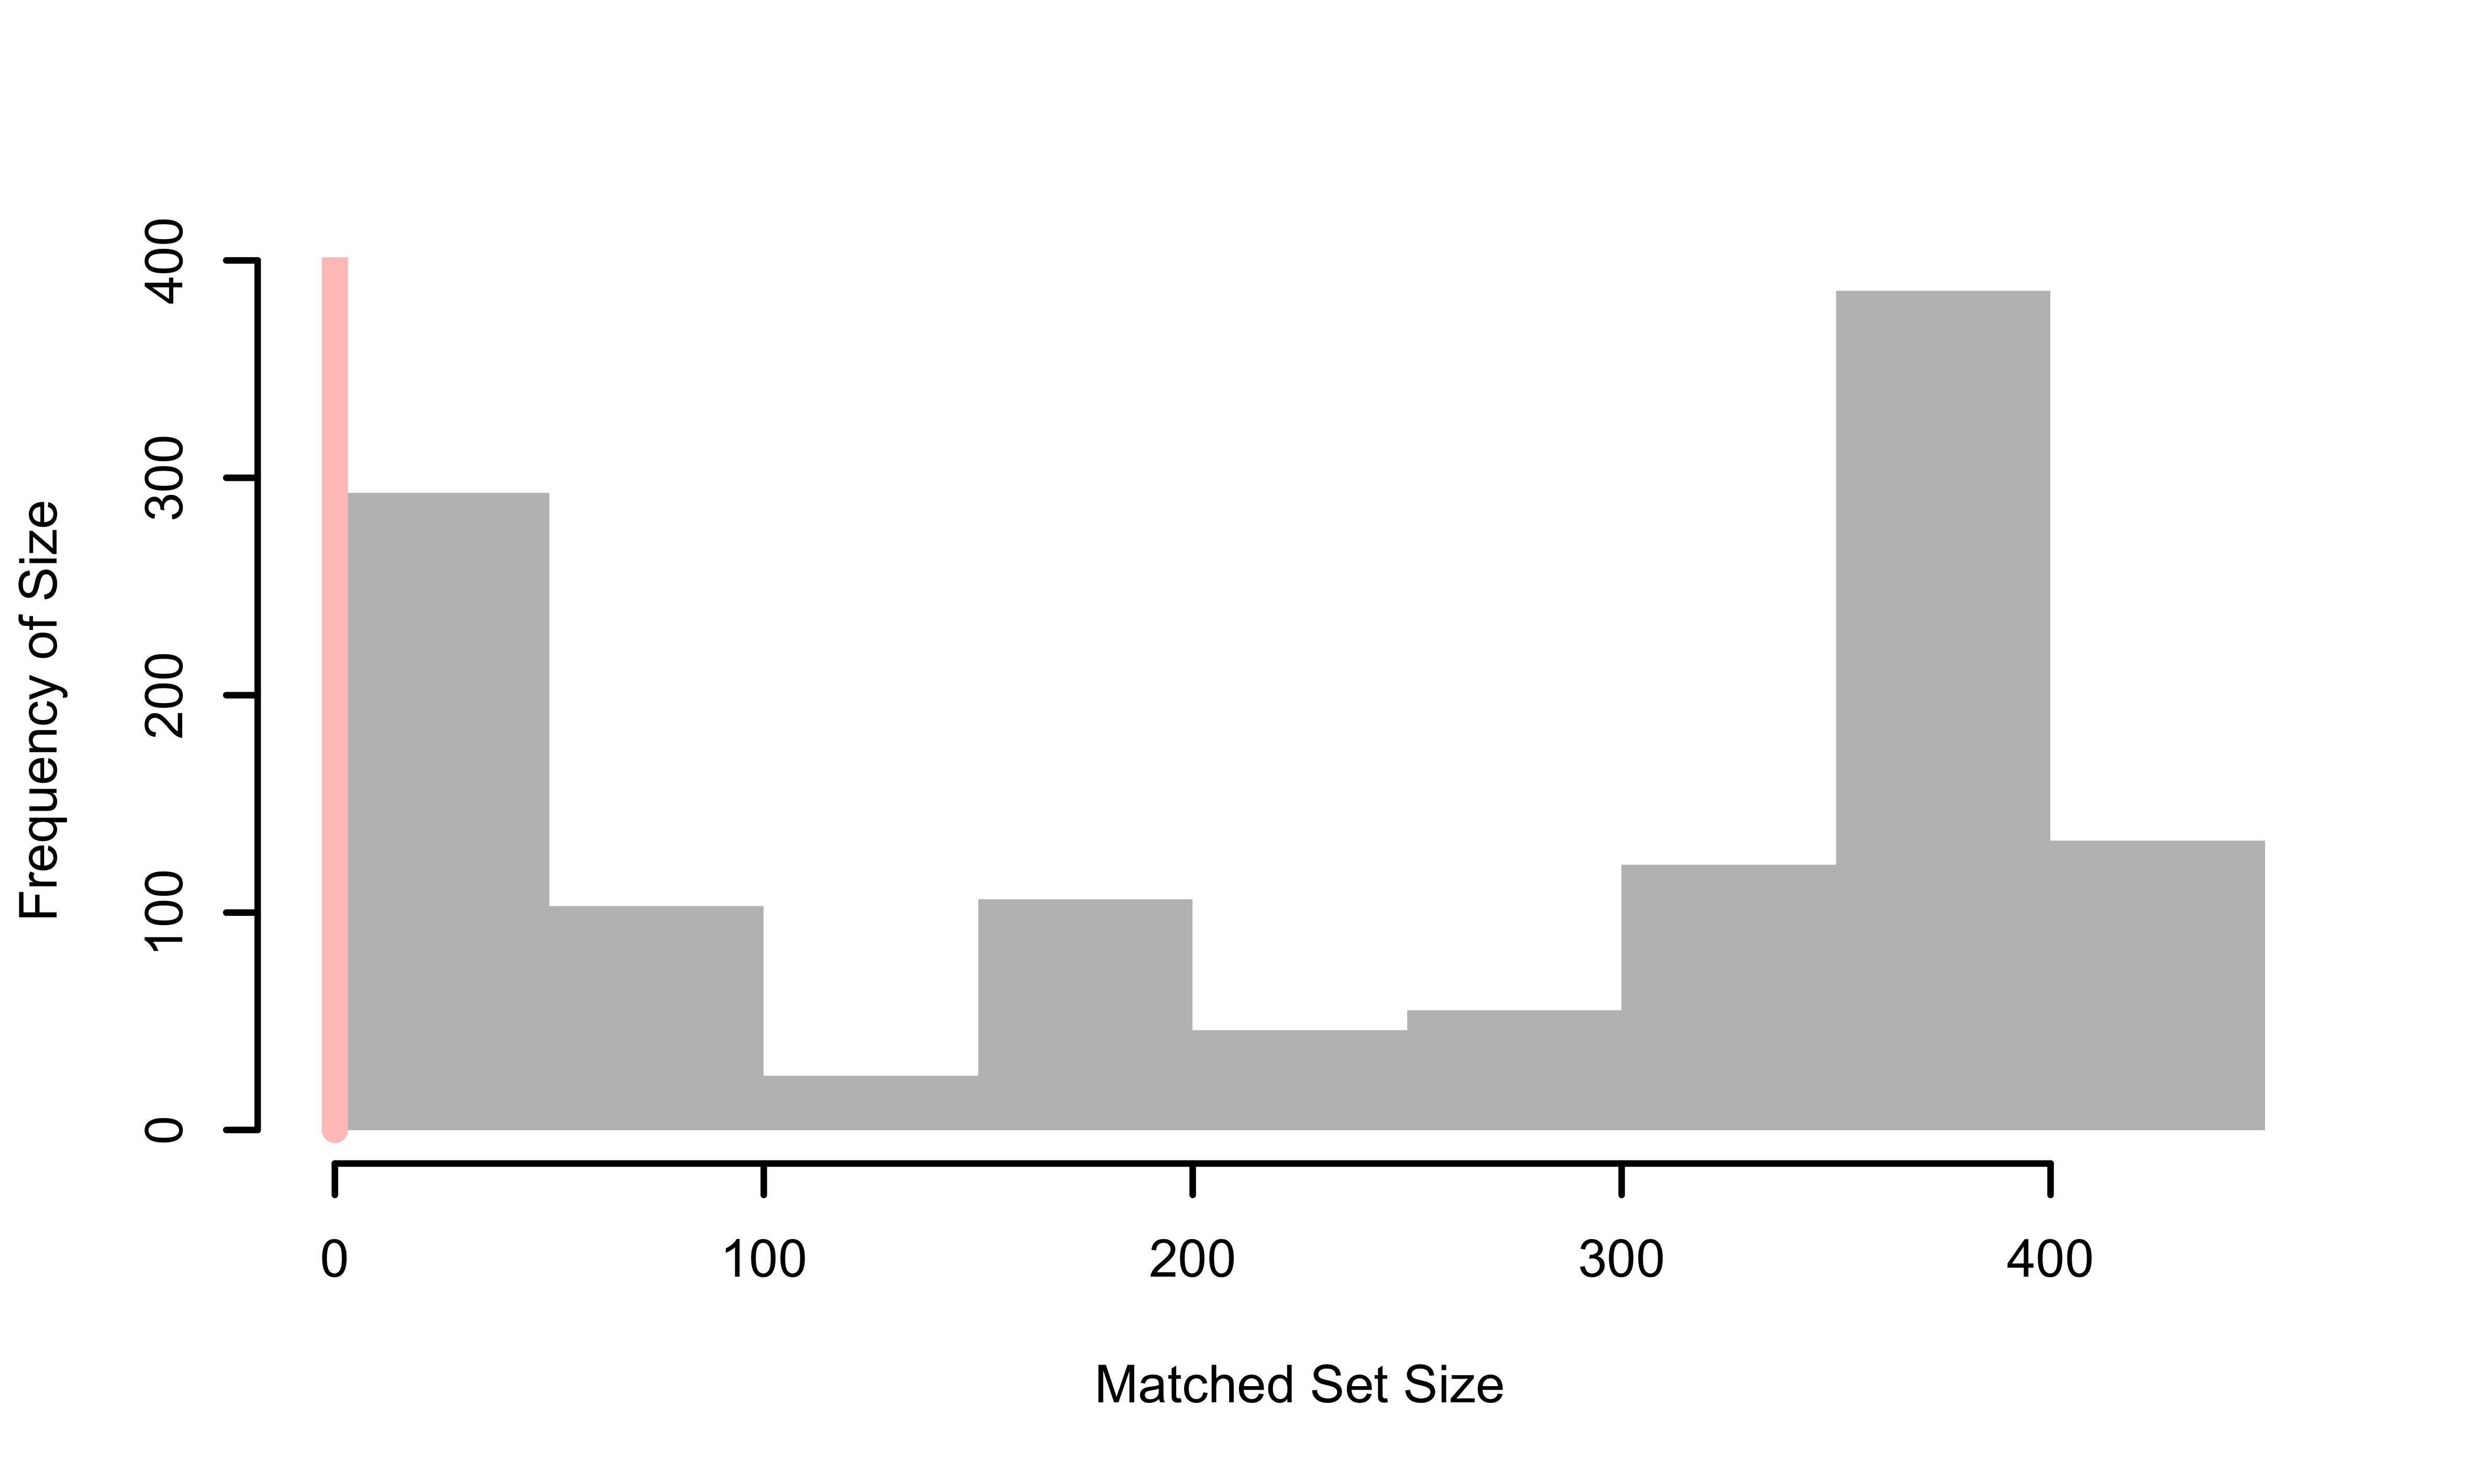
\includegraphics[width=0.8\linewidth]{\figdir/hist_matchset_size.png}
    \label{fig:hist_matchset_size}

    \fignote{\textwidth}{In the first step of the matching proceedure, each
        user gets assigned a set of potential control users that share the same
        treatment history for a specified number of periods before the user
        signs up to teh app (6 months, in our baseline specification), but that
        do not sign up themselves for a specified number of periods after the
        treatment user has signed up (another 6 months, in our baseline
        specification). The figure shows the distribution of the sizes of these
        sets of potential control users. The pink vertical bar on the left
    shows to count of users for whom no control users cound be found.}

\end{figure}

\begin{figure}[H]
    \centering
    \caption{Covariance balance}%
    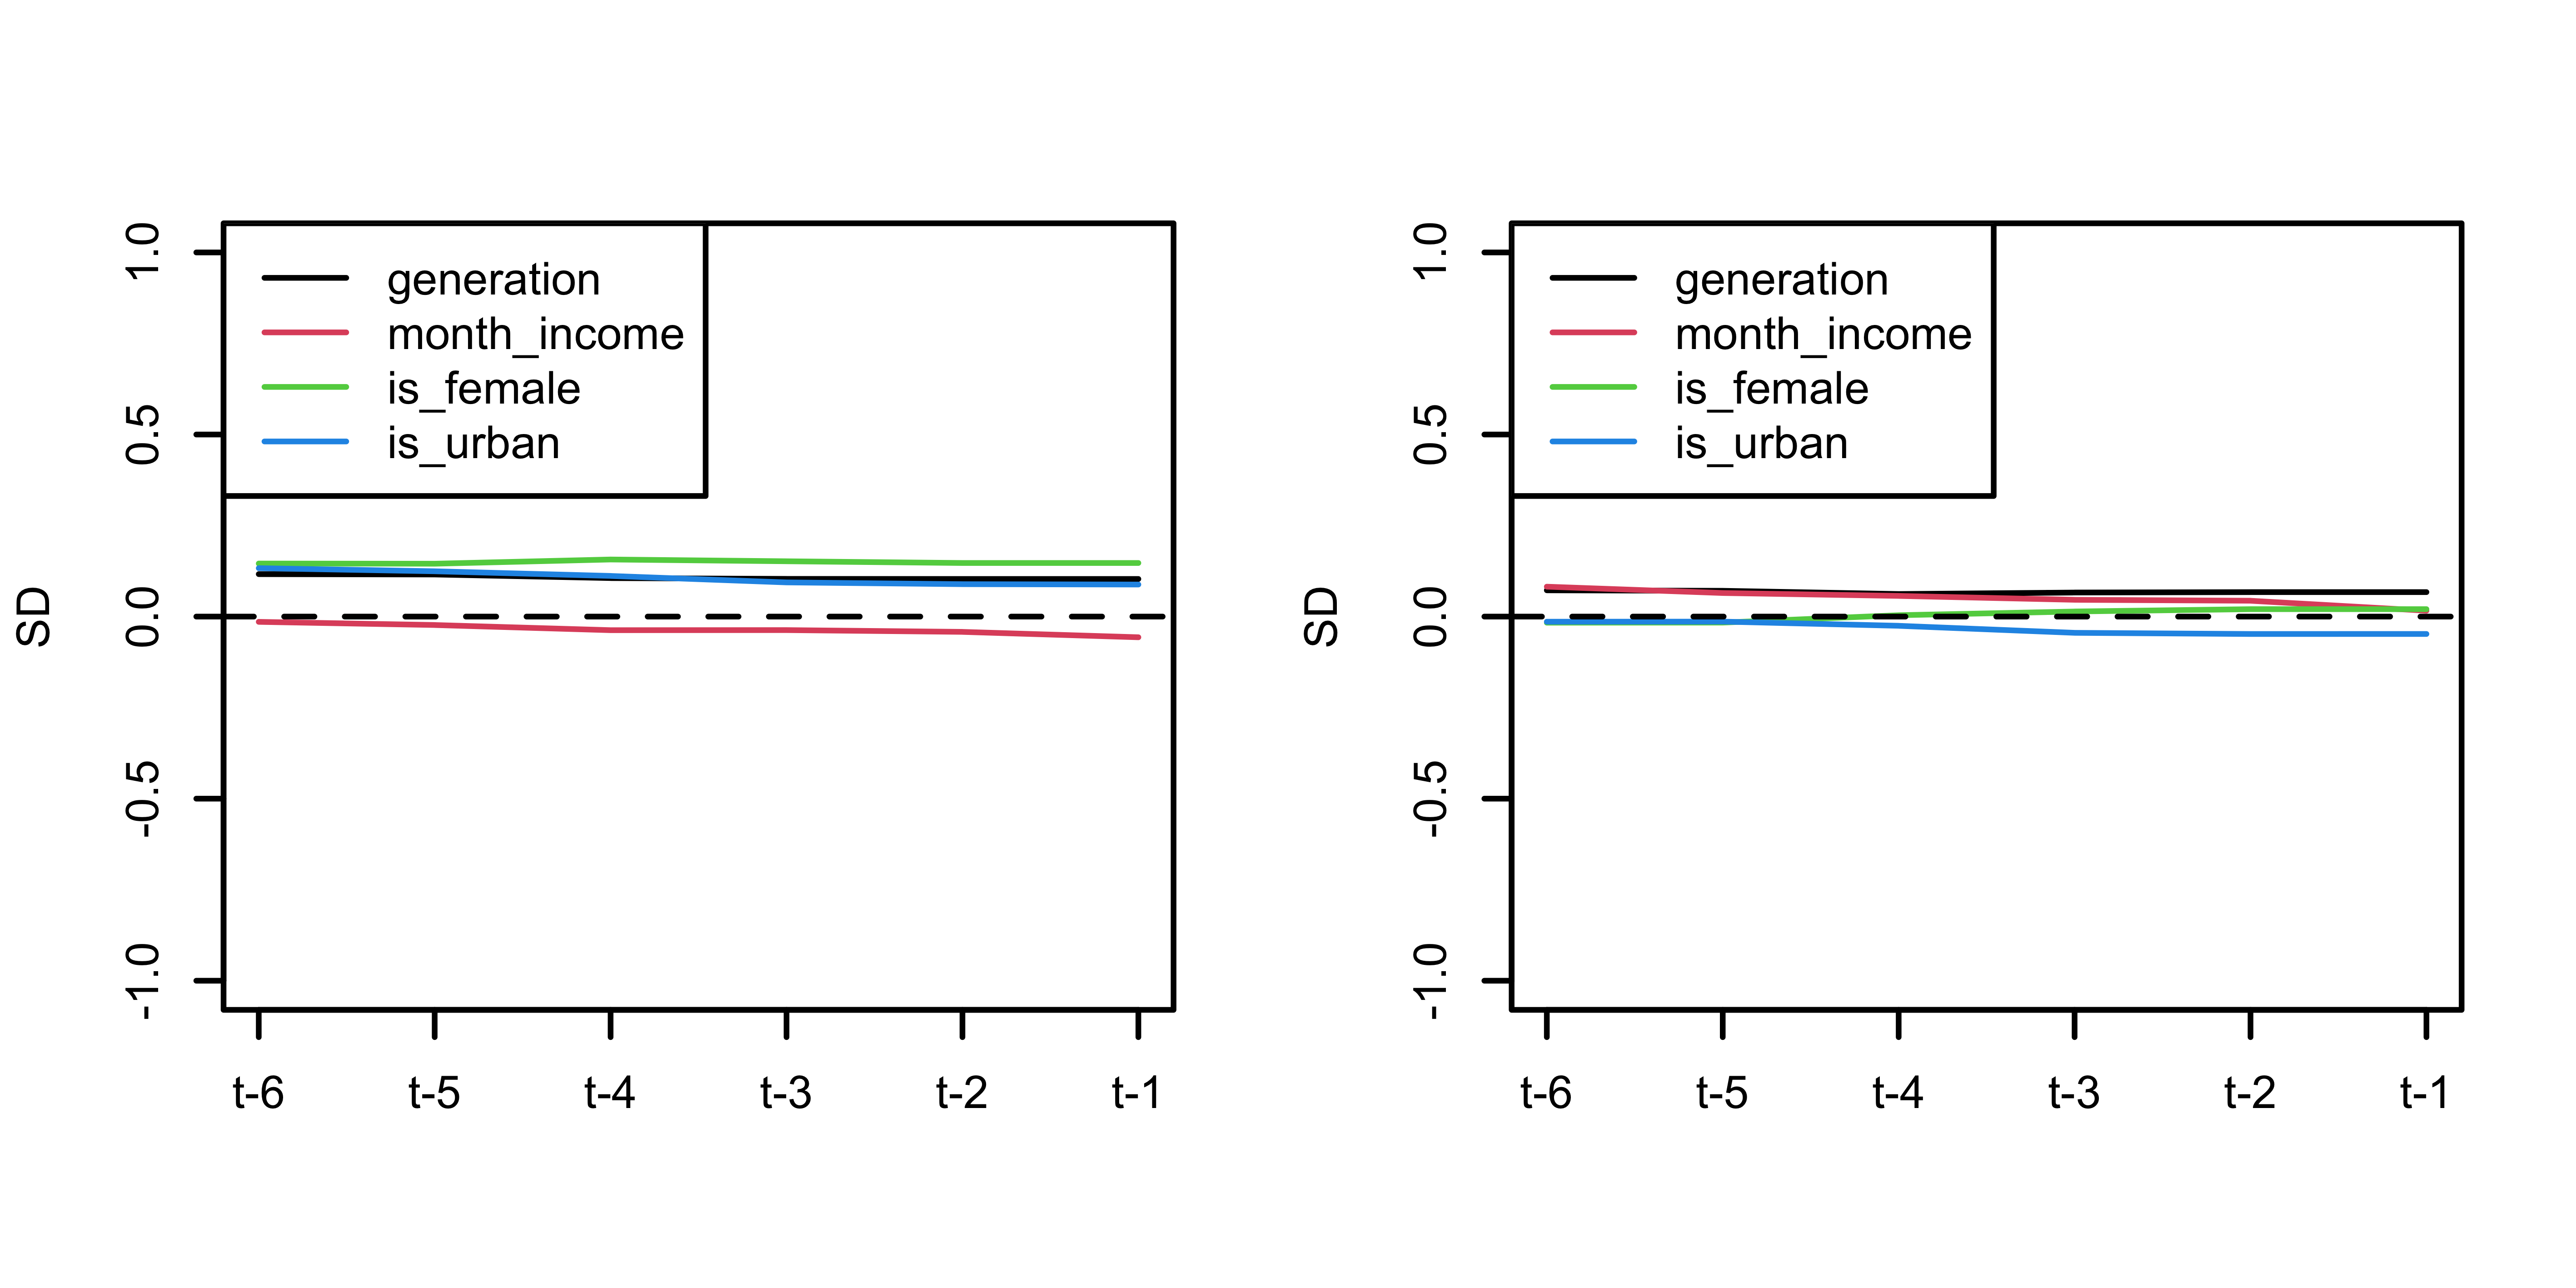
\includegraphics[width=0.8\linewidth]{\figdir/covar_balance.png}
    \label{fig:covar_balance}

    \fignote{\textwidth}{Average covariate standard deviation between treatment and
        control units for each pre-treatment period using the entire set of
        potential controls on the left and, on the right, the refined set of
        controls, which, in our baseline specification, consists of the nearest
        neighbour match based on the propensity score.}

\end{figure}

\begin{figure}[H]
    \centering
    \caption{Matching estimates}%
    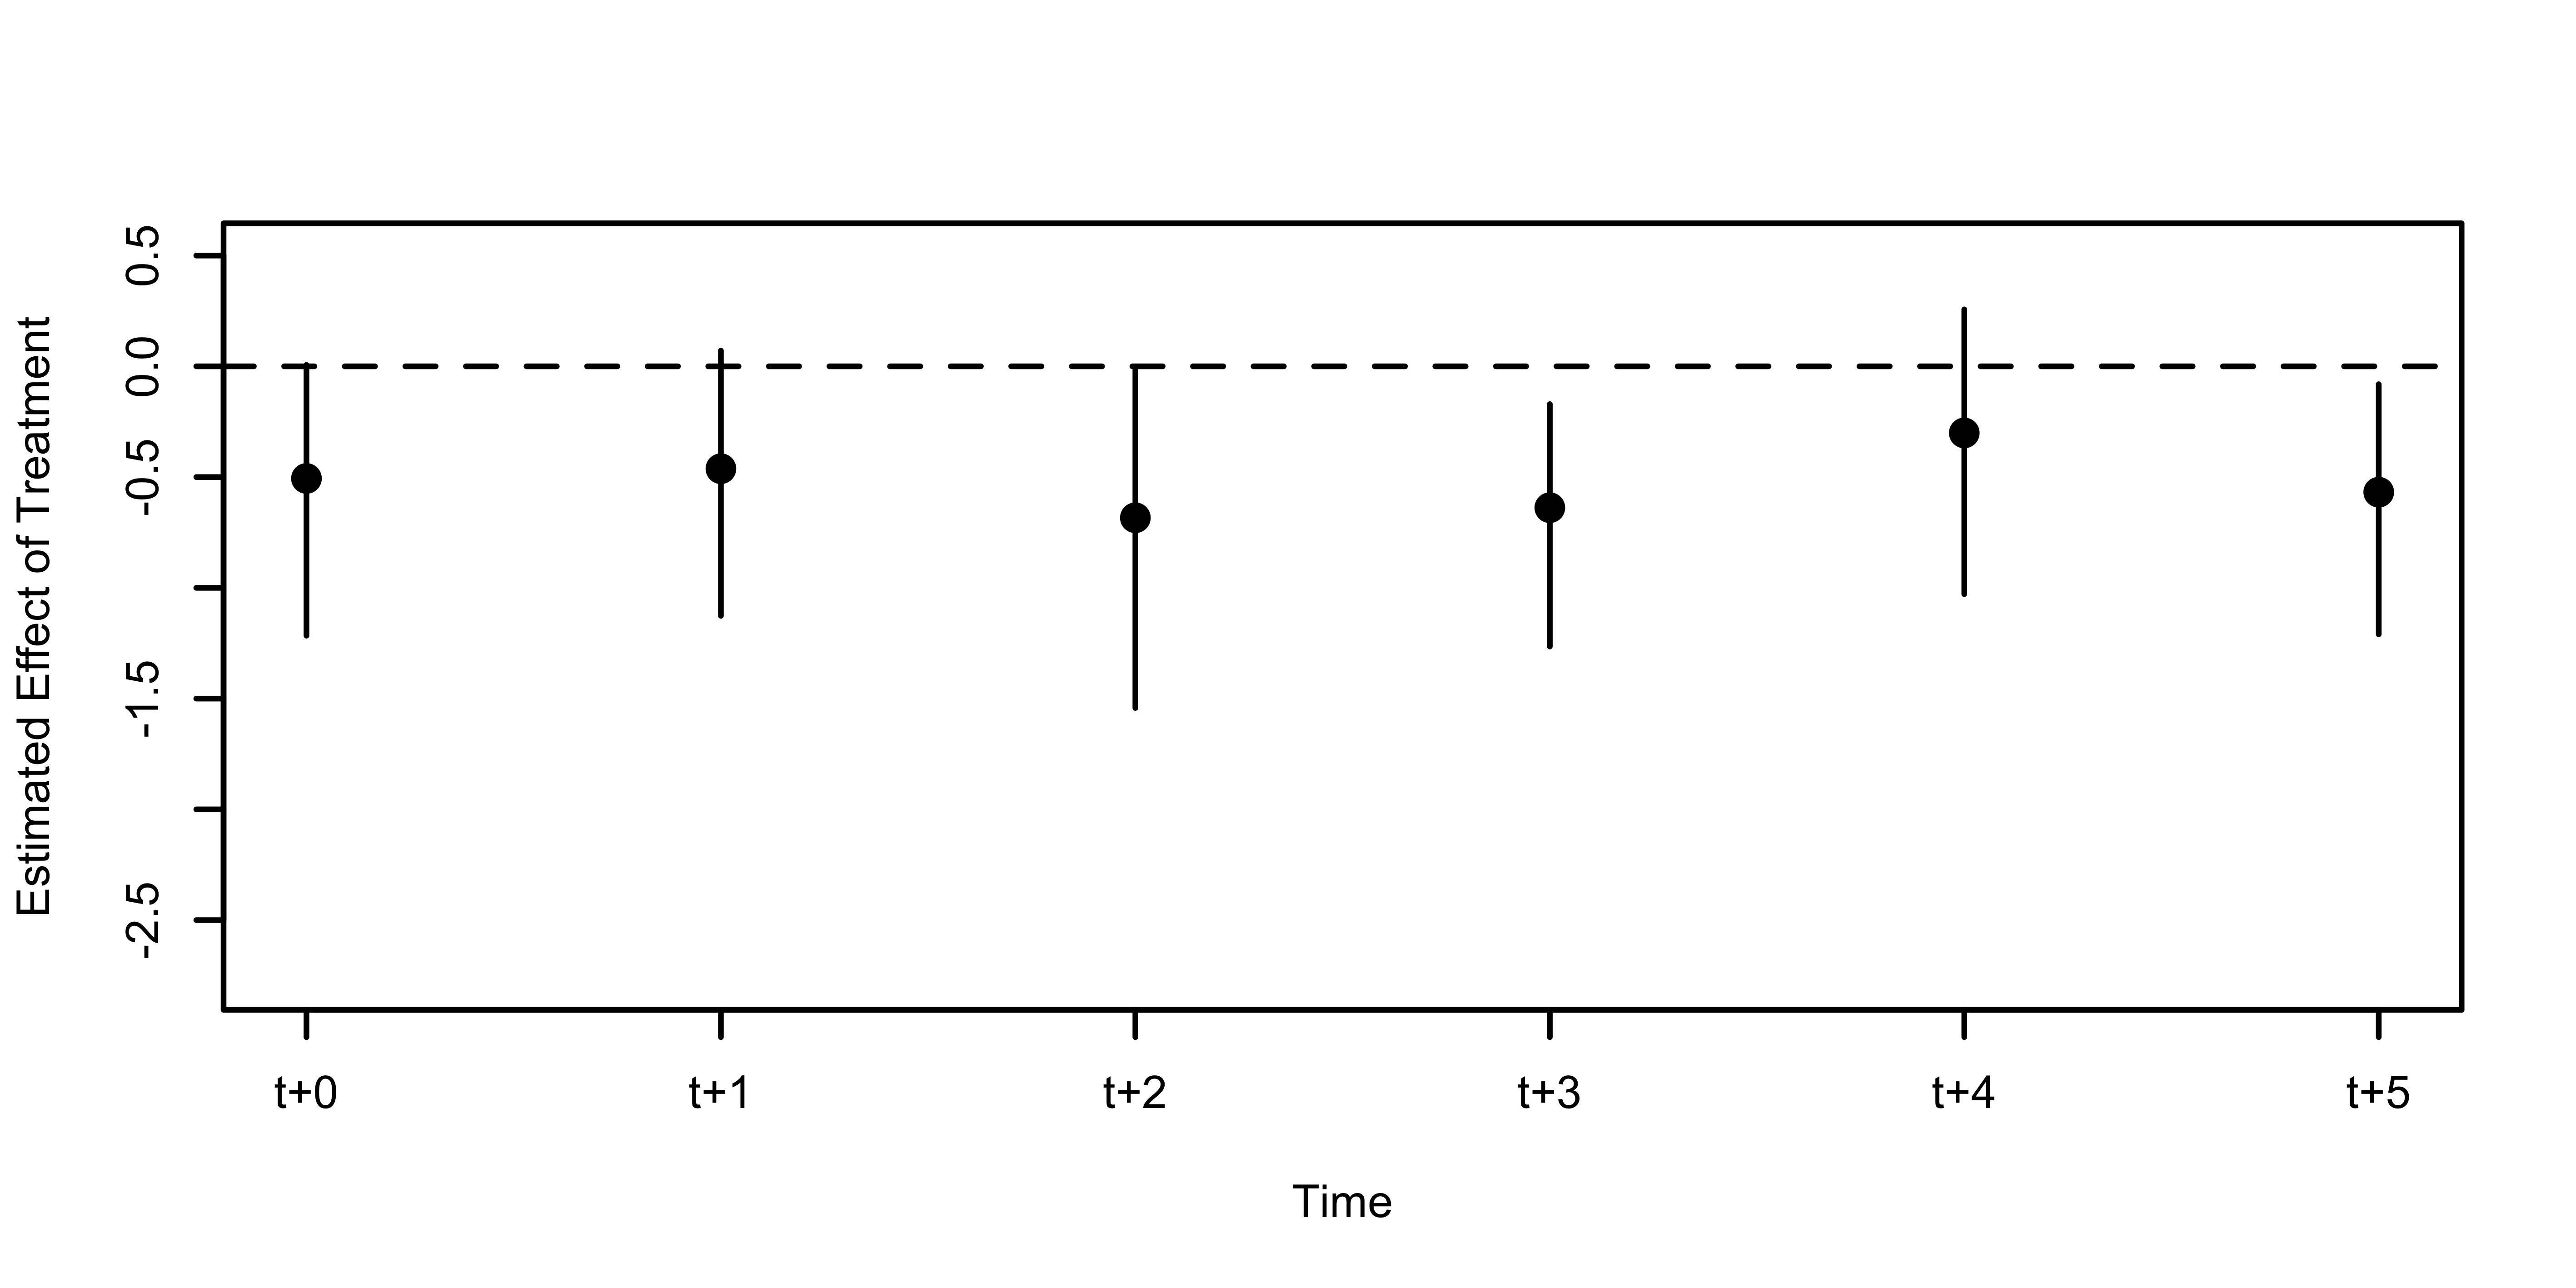
\includegraphics[width=0.8\linewidth]{\figdir/match_estimates.png}
    \label{fig:match_estimates}

    \fignote{\textwidth}{}

\end{figure}

Is estimate causal?
\begin{itemize}
    \item \citet{king2006dangers} show that there are four sources of bias
        (ommitted variable, posttreatment, interpolation, extrapolation).
    
    \item Discuss each in turn to argue that effect is causal (for our population
        of interest, which are people signing up to MDB). 
\end{itemize}


